% ╔══════════════════════════════════════════════════════════════════════╗
% ║  NLP Corpus Analysis — Group Report                                  ║
% ║  ACL Format | Text Analytics Coursework                              ║
% ╚══════════════════════════════════════════════════════════════════════╝
%
% ── HOW TO USE ────────────────────────────────────────────────────────────
%  1. Upload main.tex + references.bib + acl.sty + acl_natbib.bst to Overleaf
%  2. Upload your figures to the figures/ folder in Overleaf
%  3. Each member edits ONLY their own \begin{block}...\end{block}
%  4. Delete all \TODO{} markers before submitting
%  5. Do NOT change \documentclass, font, or margins
%
% ── PAGE BUDGET ───────────────────────────────────────────────────────────
%  Rubric:   Abstract 0.25p | Intro 1.5p | Methods 3.5p | Eval 3.5p | Concl 1p
%  Figures/tables occupy space inside these pages.
%  Estimate: every full-width figure ≈ 0.35p; every half-column figure ≈ 0.20p;
%            every small table ≈ 0.15p.
%
%  Target word counts assume ~2 pages of figures/tables across the whole paper:
%  ┌──────────────────┬──────────┬──────────────────────────────┐
%  │ Section          │ Pages    │ Target words (text only)     │
%  ├──────────────────┼──────────┼──────────────────────────────┤
%  │ Abstract         │ 0.25     │ ~160w  (Member 5)            │
%  │ Introduction     │ 1.5      │ ~800w  (all 4 share ~200w)   │
%  │ Methods          │ 3.5      │ ~1,800w (~360w per member)   │
%  │ Eval             │ 3.5      │ ~1,500w (~300w per member)   │
%  │ Conclusions      │ 1.0      │ ~600w  (~120w per member)    │
%  ├──────────────────┼──────────┼──────────────────────────────┤
%  │ Per member total │          │ ~980–1,040w                  │
%  └──────────────────┴──────────┴──────────────────────────────┘
%
% ── FIGURE FORMATTING RULES (ALL MEMBERS) ─────────────────────────────────
%  • Minimum font inside figure: 9pt (must be readable without zooming at A4)
%  • Minimum resolution: 200 dpi
%  • Prefer PDF format for vector graphics; PNG for raster
%  • Single-column figure: use {figure} environment, width=\linewidth
%  • Full-width figure:    use {figure*} environment, width=\linewidth
%  • Caption: Figure N. Brief description ending with a period.
%
%  Copy this template when inserting a figure:
%
%    \begin{figure}[t]            % use figure* for full-width
%      \centering
%      \includegraphics[width=\linewidth]{figures/YOUR_FILE.pdf}
%      \caption{Caption text.}
%      \label{fig:YOUR_LABEL}
%    \end{figure}
%
% ── TABLE FORMATTING RULES (ALL MEMBERS) ──────────────────────────────────
%  • Use booktabs: \toprule \midrule \bottomrule (no vertical lines)
%  • Font: \small inside table
%  • Caption: Table N. Brief description.
%
%  Copy this template when inserting a table:
%
%    \begin{table}[t]
%      \centering\small
%      \begin{tabular}{lcc}   % adjust columns as needed
%        \toprule
%        \textbf{Col A} & \textbf{Col B} & \textbf{Col C} \\
%        \midrule
%        row 1          & val          & val \\
%        \bottomrule
%      \end{tabular}
%      \caption{Caption text.}
%      \label{tab:YOUR_LABEL}
%    \end{table}
%
% ── CITATION RULES ────────────────────────────────────────────────────────
%  Add BibTeX entries to references.bib, then:
%    \citep{key}  →  (Author, Year)     parenthetical
%    \citet{key}  →  Author (Year)      textual
%  References section does NOT count toward the 10-page limit.
% ═══════════════════════════════════════════════════════════════════════════

\documentclass[11pt]{article}
\usepackage[review]{acl}      % sets 11pt font, 2.5cm margins automatically
\usepackage{times}
\usepackage{latexsym}
\usepackage{microtype}
\usepackage{graphicx}
\usepackage{booktabs}
\usepackage{amsmath}
\usepackage{xcolor}

\graphicspath{{figures/}}
\bibliographystyle{acl_natbib}

% Helper commands — DELETE before submitting
\newcommand{\TODO}[2]{\noindent\textcolor{red}{\textbf{[#1]}}\textcolor{gray}{\small\textit{ (~#2 words)}}\medskip}
\newcommand{\WC}[1]{\noindent\textcolor{gray}{\footnotesize[Target: #1 words]}\smallskip}

% ═══════════════════════════════════════════════════════════════════════════
\title{How Has NLP Research Changed? \\
A Comparative Corpus Analysis of arXiv Abstracts, 1991--2021}

\author{%
  Member 1 \quad Member 2 \quad Member 3 \quad Member 4 \quad Member 5 \\
  Text Analytics Coursework}

\begin{document}
\maketitle

% ═══════════════════════════════════════════════════════════════════════════
% ABSTRACT   Target: ~160 words | Owner: Member 5 | Write LAST
% ═══════════════════════════════════════════════════════════════════════════

\begin{abstract}

Scientific abstracts show how researchers framing problems and key findings. We study how this framing has changed in NLP by analysing 32,221 arXiv cs.CL abstracts spanning 1991 to 2021. Two analytical axes structure the project: Axis-1 compares four representation methods (TD-IDF unigrams, TF-IDF bigrams, SBERT embeddings, and LDA topic distributions), and Axis-2 compares two temporal comparison methods (keywords shift analysis and cosine distance between period centroids). Centroid trajectories are visualised through PCA and UMAP projections. All four Axis-1 methods agree on a single dominant breakpoint from 2011-2015 to 2016-2021 transition, which is consistent with the rise of transformer-based pre-training. The Axis-2 cosine distance results uncover a layered pattern beneath this consensus: lexical change peaks first, semantic change later, and topical change last. NLP's paradigm shift propagated upward through representational layers instead of occurring simultaneously. 

\end{abstract}




% ═══════════════════════════════════════════════════════════════════════════
% 1. INTRODUCTION   Target: ~800 words total | ~200 words per member
%    Rubric: task, motivations, data, requirements, optional examples/plots
% ═══════════════════════════════════════════════════════════════════════════
\section{Introduction}
\label{sec:intro}

% ── Member 1: Task and motivation ─────────────────────────────────────────
% Why studying the evolution of NLP research framing matters.
% End with the explicit research question this project answers.


Over the past three decades, Natural Language Processing (NLP) has undergone major paradigm shifts, from rule-based and statistical approaches to data-driven machine learning and transformer-based models recently. These transitions are well documented in terms of performance, motivating a data-driven exploration of how research focus evolves over time.

Scientific abstracts provide a concise and standardised representation of research output, making them suitable for tracking such changes at scale. Analysing lexical and semantic patterns in abstracts could offer a perspective on the evolution of research focus and discourse.

In terms of shifts in vocabulary, for example, from grammar and parsing to neural and pre-trained, indicating not only new techniques but changing conceptualisations of NLP. Identifying when these shifts occur and whether different analytical methods capture them consistently could provide insight into the dynamics of scientific change.

This project addresses the question of how the focus and vocabulary of NLP research have evolved over time and how methodological choices influence the insights obtained.


% ── Member 2: Available data ──────────────────────────────────────────────
% Describe the corpus: source, size, time range, period binning,
% and any notable characteristics (e.g. class imbalance).
% Add a data exploration figure or table here if you wish.
The source corpus was the public and available \texttt{gfissore/arxiv-abstracts-2021} dataset, which provides arXiv metadata and abstracts up to the end of 2021. From this larger collection, NLP-related articles were filtered using the arXiv subject labels \texttt{cs.CL} and \texttt{cmp-lg}. To support the comparison in different periods, the publication year was extracted on the basis of the arXiv identifier, and records without reliable year information were excluded. The filtered NLP corpus contains 32,221 abstracts covering 1994--2021.

For historical comparison, the filtered corpus was grouped into six period bins: 1991--1995, 1996--2000, 2001--2005, 2006--2010, 2011--2015, and 2016--2021. As shown in Table~\ref{tab:corpus-summary}, the first bin is labeled 1991--1995, but the earliest year of retained records in the filtered corpus is 1994. A distinguishable characteristic of the corpus is its strong temporal imbalance, as the number of abstracts in the 2016--2021 period is much higher than in all previous periods, representing approximately 88.16\% of the corpus. From Figure~\ref{fig:period-counts}, it is clear that the overwhelming majority of abstracts are concentrated in the 2016--2021 period, while the earlier bins are comparatively small.

\begin{table}[t]
\centering
\small
\begin{tabular}{lrrrr}
\hline
Period & Count & Year min & Year max & Era \\
\hline
1991--1995 & 448   & 1994 & 1995 & Statistical Methods \\
1996--2000 & 659   & 1996 & 2000 & Statistical Methods \\
2001--2005 & 279   & 2001 & 2005 & Machine Learning \\
2006--2010 & 364   & 2006 & 2010 & Machine Learning \\
2011--2015 & 2066  & 2011 & 2015 & Deep Learning \\
2016--2021 & 28405 & 2016 & 2021 & Transformer \& Pre-training \\
\hline
\end{tabular}
\caption{Statics of the filtered NLP corpus.}
\label{tab:corpus-summary}
\end{table}

\begin{figure}[t]
\centering
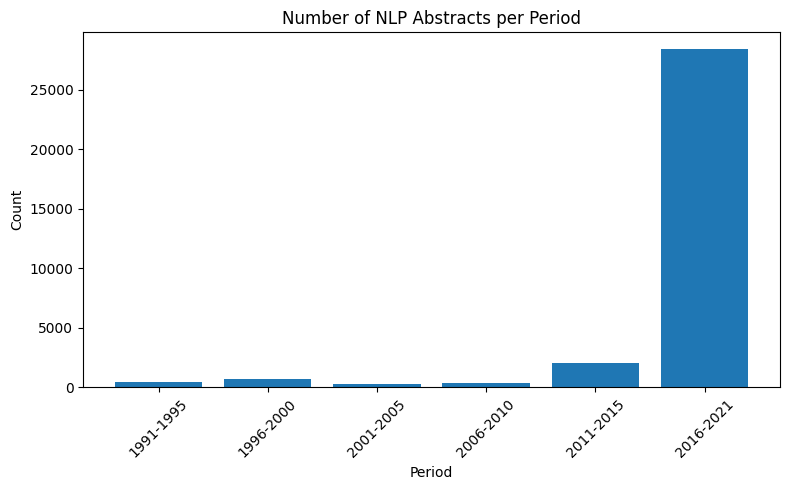
\includegraphics[width=0.9\linewidth]{figures/period_counts.png}
\caption{Number of NLP abstracts per period.}
\label{fig:period-counts}
\end{figure}

% ── Member 3: Requirements for a good solution ───────────────────────────
% What properties must a method have to answer the research question well?
% Use these requirements to motivate the two analytic axes.
% ── Member 3: Requirements for a good solution ───────────────────────────
A reliable method for tracking change in NLP research must meet 
four requirements. First, it must be interpretable: the output 
should point directly to specific words or phrases, not just 
numerical scores that require further explanation. Second, it 
must account for corpus imbalance: because the 2016--2021 period 
contains far more abstracts than earlier periods, any comparison 
must normalise for period size to avoid mistaking quantity for 
significance. Third, it must capture both directions of change: 
identifying not only which terms became prominent but also which 
terms disappeared from the research vocabulary. Fourth, it must 
be transparent enough for readers to verify the findings without 
specialist tools. These four requirements motivate the two analytic 
axes in this study. Axis 1 examines how the choice of text 
representation of TF-IDF versus semantic embeddings shapes 
what patterns become visible. Axis 2 examines how the choice of 
comparison method, keyword shift analysis versus cosine 
distance determines what kind of change can be detected 
and explained.




% ── Member 4: Dataset examples ────────────────────────────────────────────
% Paraphrase one or two concrete abstracts (early vs late) to show the reader
% what the vocabulary shift looks like. Add a figure if helpful.
%\TODO{Member 4 — Dataset examples (~200w).
%Paraphrase one early (1991--2005) and one recent (2016--2021) abstract.
%Identify 2--3 concrete differences in framing and vocabulary.
%A figure illustrating the vocabulary shift is optional but encouraged.}{200}

The vocabulary difference when compared between early and recent NLP abstracts shows how the field transformed over time. A 1994 paper on tree adjoining grammars focuses on derivation trees, syntactic analysis, linear indexed grammars and parsing algorithms, which showed NLP as a problem of linguistic structure and computational grammar. The research question is framed in terms of correctness of linguistic structure rather than measurable accuracy on benchmark datasets.

On the other hand, a 2018 paper about Universal Language Model Fine-tuning (ULMFiT) talks about inductive transfer learning, pre-trained models, fine-tuning and state of the art performance on benchmark datasets. The research question is framed with respect to generalization across tasks and reduction in data requirements, which were absent in the 1994 abstract.

Three differences can be noted from the above comparison. First, the interest of analysis transformed from grammatical structures to neural model parameters. Second, the evaluation criteria shifted from linguistic correctness to measurable accuracy. Third, the framing of contribution shifted from theoretical reformulation to practical transfer and generalization. The above differences shows the two analytic axes in this study of whether text representation methods and comparison methods can characterize this transformation systematically across all 32,221 abstracts.
% ═══════════════════════════════════════════════════════════════════════════
% 2. METHODS   Target: ~1,800 words total | ~360 words per member
%    Rubric 3a: baseline + preprocessing + representations
%    Rubric 3b: axes of experimentation
%    Rubric 3c: proposed improvements + hypotheses
% ═══════════════════════════════════════════════════════════════════════════
\section{Methods}
\label{sec:methods}

% ── Member 1: Preprocessing and TF-IDF baseline (Rubric 3a) ──────────────
% Describe the preprocessing pipeline (NB00) and the TF-IDF baseline.
% Include the TF-IDF equation. State vocabulary sizes.
% Justify design choices. Add a figure if it clarifies the pipeline.
\TODO{Member 1 — Preprocessing + TF-IDF baseline (~360w, Rubric 3a).
Cover: pipeline overview, preprocessing steps (lowercasing, tokenisation,
stopword removal, etc.), TF-IDF unigram baseline (include Eq.~1, vocabulary
size, hyperparameters), TF-IDF bigram as first axis alternative.
Justify each choice.}{360}

\subsection{Data Preparation and Preprocessing}


The dataset was filtered from 1999486 abstracts to retain papers categorised under \texttt{cs.CL} and \texttt{cmp-lg}, resulting in 32221 abstracts from 1994 to 2021, with the inclusion of \texttt{cmp-lg}, the predecessor of \texttt{cs.CL}. It ensures coverage of early NLP research and avoids discontinuities in the dataset. Publication years were extracted from both legacy and modern arXiv identifier formats, and documents were grouped into six five-year periods (1991-1995 to 2016-2021) to ensure comparability across time, with 2021 merged into the final bin due to limited sample size. Each period was further associated with a corresponding NLP technical paradigm for interpretation.


Text preprocessing involved lowercasing, removal of non-alphabetic characters, stopword filtering, and lemmatisation to reduce noise and improve consistency across documents.

\subsection{TF-IDF Representations}

TF-IDF Unigram was adopted as a baseline representation due to its minimal assumptions and direct interpretability, enabling transparent comparison of lexical importance across periods. Representations were generated using \texttt{min\_df=5} and \texttt{max\_df=0.85} to remove noise and overly common terms, with \texttt{sublinear\_tf=True} to reduce the dominance of high-frequency tokens, resulting in a vocabulary of approximately 15000 terms. Given the substantial imbalance in document counts across periods, term importance was aggregated by the mean rather than the sum. We hypothesise that TF-IDF Unigram will capture broad lexical shifts between paradigms, for instance, the decline of statistical terminology and the rise of neural vocabulary. However, it tends to treat semantically related terms with different surface forms as unrelated, thereby limiting its ability to capture deeper connections in meaning.



TF-IDF Bigram extends the baseline by capturing compound expressions such as language model and neural network, which are not preserved in unigram representations. Using the same parameter settings, the bigram vocabulary contains approximately 18000 terms. For each period, top-ranked terms were extracted to identify emerging and declining vocabulary. For the vocabulary shift comparison, periods were divided into early (1991-1995, 1996--2000, 2001-2005) and late (2011-2015, 2016-2021). The 2006-2010 period here was excluded from this binary comparison as a transitional interval whose mixed vocabulary profile would obscure the contrast between the two paradigms. We hypothesise that TF-IDF Bigram will identify paradigm-specific compound terms, such as pre-trained model and attention mechanism that unigram representations fail to capture, providing a more precise characterisation of how NLP concepts are expressed across periods while remaining interpretable.




% ── Member 2: Semantic representations (Rubric 3a + 3c) ──────────────────
% Describe SBERT and LDA as proposed improvements over TF-IDF.
% State hypotheses about how each will perform differently.

\subsection{SBERT and LDA Representations}

Based on the TF-IDF baseline, two additional non-lexical text representations were introduced to capture patterns that the lexical overlap alone may miss. While TF-IDF Unigram and TF-IDF Bigram represent abstracts through observable word and phrase frequency, SBERT and LDA, respectively, encode text from the two levels of sentence meaning and thematic structure. Therefore, they are used not as replacements for TF-IDF, but as complementary representations to testing whether the historical development of NLP appears different once the lexical form is separated from the deeper semantic or topical organization.

SBERT was implemented with the \texttt{all-MiniLM-L6-v2} Sentence-Transformers model, which maps each abstract to a d384-dimensional dense vector \citep{allminilm_modelcard}. With the complete cleaned data(32221), SBERT produced an embedding matrix of shape \texttt{(32221, 384)}. Sentence-BERT is based on siamese BERT networks trained to place semantically similar texts close together in vector space, making it suitable for semantic similarity and clustering tasks \citep{reimers2019sentence}. Unlike TF-IDF, SBERT can capture shifts in meaning even when related research is expressed through different lexical choices. Therefore, it is hypothesized that SBERT will reveal a long-range semantic drift that remains partially invisible to TF-IDF, especially in cases where terms change without completely disrupting the underlying research content.

LDA was used to model the thematic structure at the corpus level\citep{blei2003latent}. After token-based filtering, 32,217 abstracts remained for topic modeling and the resulting dictionary contained 12,860 terms. Each abstract was represented as a topic-proportion vector, where each dimension corresponds to the probability weight of a latent topic. Candidate values of $K=8$, $K=10$, and $K=15$ were compared using coherence, generating scores of 0.5101, 0.5082, and 0.5127, respectively; $K=15$ was selected as the final topic number. This higher value was preferred because it achieved the strongest coherence while still producing interpretable topics such as translation, embeddings, transformers, speech recognition, parsing, sentiment analysis, and knowledge graphs. The hypothesis is that LDA will reveal structural reorganization in research themes more clearly than TF-IDF, because it groups related vocabulary into shared latent topics instead of treating words independently.

% ── Member 3: Keyword shift axis (Rubric 3b + 3c) ────────────────────────
% Describe the keyword shift comparison method.
% State a clear hypothesis about what it will reveal.
Keyword shift analysis tracks vocabulary change by identifying which terms are most prominent in each time period and comparing those lists across periods. For each of the six five-year bins, the mean TF-IDF score is computed across all abstracts in that period. The mean is used rather than the sum to account for the strong temporal imbalance in the corpus, ensuring scores remain comparable across periods of different sizes.

The top-$N$ terms are extracted after filtering a custom stoplist of generic academic phrases, including paper, based, used, and present, which appear consistently across all periods without reflecting genuine research content. $N$ is set to 20. The analysis is run separately for unigrams and bigrams to capture both individual terms and compound concepts such as language model and neural network.

For the vocabulary shift comparison, periods were divided into early (1991--1995, 1996--2000, 2001--2005) and late (2011--2015, 2016--2021). The 2006--2010 period was excluded from this binary comparison as a transitional interval whose mixed vocabulary profile would obscure the contrast between the two paradigms.

Emerging vocabulary is defined as terms present in the top-$N$ lists of both late periods but absent from all three early periods. Disappearing vocabulary is defined symmetrically. The hypothesis is that keyword shift analysis will identify the specific vocabulary items responsible for the observed change in NLP research, something that cosine distance and embedding-based methods cannot do by design. While cosine distance measures how much two periods differ as a whole, keyword shift produces directly readable evidence: a named list of terms that rose and a named list that fell.


% ── Member 4: Cosine distance axis (Rubric 3b + 3c) ──────────────────────
% Describe the cosine distance comparison method.
% State a clear hypothesis about what it will reveal.

\subsection{Axis 2B: Cosine Distance}
\label{sec:methods-axis2}

Cosine distance analysis measures the magnitude of change between time periods by comparing their centroid vectors in the representation space. For each time period, a centroid is computed by taking the mean of all abstract vectors within that period:

\begin{equation}
    \mathbf{c}_p = \frac{1}{|P|} \sum_{i \in P} \mathbf{v}_i
\end{equation}

where $\mathbf{c}_p$ is the centroid of period $p$, $P$ is the set of abstracts in that period, and $\mathbf{v}_i$ is the vector representation of abstract $i$. The cosine distance between two adjacent period centroids is then computed as:

\begin{equation}
    d(p_1, p_2) = 1 - \frac{\mathbf{c}_{p_1} \cdot \mathbf{c}_{p_2}}{\|\mathbf{c}_{p_1}\| \|\mathbf{c}_{p_2}\|}
\end{equation}

Cosine distance is well suited to high-dimensional text vectors because it measures the angle between vectors rather than their absolute distance. This makes it invariant to vector magnitude - a period with more abstracts does not produce a larger centroid simply because more vectors were averaged. This property is particularly important given the strong temporal imbalance in this corpus, where the 2016-2021 period contains 88\% of all abstracts.

This method differs fundamentally from keyword shift analysis in what it can reveal. Keyword shift identifies which specific terms changed and in which direction - it produces a named list of rising and falling vocabulary items. Cosine distance instead measures how much the overall representation of a period changed relative to the previous one, without identifying the specific terms responsible. The two methods are therefore complementary: keyword shift provides interpretable evidence of what changed, while cosine distance provides a quantitative signal of when and how dramatically the change occurred.

The analysis was applied to all four representations - TF-IDF unigram, TF-IDF bigram, SBERT and LDA - producing four independent distance timelines. Comparing these timelines tests whether different representation choices lead to different conclusions about the timing of NLP's major paradigm shifts. We hypothesize that TF-IDF based distances will detect the earliest breakpoint since vocabulary change is a surface level signal that precedes deeper conceptual shifts. SBERT distances are expected to detect a later breakpoint, reflecting when the semantic meaning of research fundamentally changed rather than just its terminology. LDA distances are expected to show the most gradual change overall, since broad research topics shift more slowly than individual words or semantic representations. If this cascade pattern holds across all four representations it would suggest that NLP's paradigm shift was a gradual process rather than a sudden revolution - surface vocabulary changed first, followed by semantic meaning, followed by a full reorganization of research topics.

% ── Member 5: Dimensionality reduction design (Rubric 3a + 3c) ───────────
% Describe PCA and UMAP as visualisation methods.
% Justify the two-stage SVD→PCA pipeline for TF-IDF.
% State a hypothesis comparing PCA and UMAP.
\subsection{Dimensionality Reduction: PCA and UMAP}
\label{sec:methods-dr}

In order to visually and quantitatively compare the four Axis-1 representations in Section~\ref{sec:methods} and Section~\ref{sec:methods-axis2}, each representation method must be projected on a two-dimensional plane. The right strategy depends on the structure of the source matrix. 

%\paragraph{The two-step TF-IDF processing flow.}

If PCA is performed on the TF-IDF matrix, the entire sparse matrix must be transformed into a dense table. However, due to memory limitations, this is not possible for the size of our data set. Therefore, we adopted a two-step approach that follows the latent semantic analysis (LSA) framework proposed by \citet{deerwester1990indexing}.The first step is to directly manipulate the sparse format with \texttt{TruncatedSVD}, reducing the dimensionality of each matrix to 50 dense dimensions. The cumulative variance grows smoothly as a function of ~$k$: When $k{=}50$, the cumulative explained variance of the unigrams reaches 11.6\%, while the cumulative explained variance of the bigrams reaches 4.5\%. For high-dimensional sparse text data, the information is widely distributed in thousands of lexical dimensions \citep{deerwester1990indexing}, so that no turning point is expected. According to the standard practice of LSA, we set $k{=}50$. In the second step, PCA reduces the dimensional output 50 to two dimensions. For unigrams, the effective variance retained is  PC1\,=\,0.64\% and PC2\,=\,0.56\%, while for bigrams they are PC1\,=\,0.22\%, PC2\,=\,0.21\%, both expressed as a percentage of the initial total variance.

%\paragraph{Direct PCA for dense matrices.}

Due to the high density of SBERT embeddings (384 dimensions) and LDA topic distributions (15 dimensions), the standard PCA was applied directly. The total explained variance of SBERT is 10.45\%, while the LDA reaches 40.22\%. The significantly hight LDA values reflect its inherent lower dimensions: with only 15 topic dimensions, PCA captured a significant share of the total structure in the first two components (PC1\,=\,26.6\%, PC2\,=\,13.7\%).

%\paragraph{UMAP as an alternative nonlinear method.}

To access whether the linear projection of PCA distorts the time structure, we also applied UMAP \citep{mcinnes2018umap-software}, a non-linear manifold method that preserves the local neighborhood topology. For the TF-IDF matrix, the treatment is SVD (50)\,$\to$\,L2-normalise\,$\to$\,UMAP (cosine); for SBERT we applied UMAP (cosine) directly; for LDA we use UMAP(euclidean) to match the simple geometric structure of the proportions of the subject. We always set \texttt{n\_neighbors}\,=\,30 and \texttt{min\_dist}\,=\,0.3. And set \texttt{random\_state}\,=\,42 to ensure repeatability. Our hypothesis is that PCA will reveal clearer and more directly comparable trends among the four representations of Axis-1, while UMAP will highlight the local subdomain structure ignored by linear projection.

% ═══════════════════════════════════════════════════════════════════════════
% 3. EXPERIMENTAL EVALUATION   Target: ~1,500 words total | ~300w per member
%    Rubric 4a: metrics and their limitations
%    Rubric 4b: experimental setup
%    Rubric 4c: results with interpretation
%    Rubric 4d: error analysis
%    Rubric 4e: discussion, strengths/limitations, recommendations
% ═══════════════════════════════════════════════════════════════════════════
\section{Experimental Evaluation}
\label{sec:eval}

% ── Member 1: Axis 1 TF-IDF results (Rubric 4a + 4b + 4c + 4d) ──────────
% Report and interpret the TF-IDF trajectory results.
% Include figures and/or tables you think best present these findings.
% Analyse errors or patterns where TF-IDF produces unexpected results.
\TODO{Member 1 — Axis 1 TF-IDF results (~300w, Rubric 4a--4d).
State the metric(s) you use and their limitations for TF-IDF trajectories.
Describe how hyperparameters were set.
Present your main TF-IDF findings (add a figure or table if helpful).
Identify patterns where TF-IDF produces misleading or surprising results.}{300}
\subsection{TF-IDF Analysis}

TF-IDF scores are used as the primary metric to track vocabulary trajectories across time, where term importance is measured by relative frequency weighted by inverse document frequency. To account for the imbalance in document counts across periods, term importance is aggregated using the mean rather than the sum. The representations are constructed using \texttt{min\_df=5}, \texttt{max\_df=0.85}, \texttt{max\_features=20000} and \texttt{sublinear\_tf=True}, which reduce noise from rare and overly frequent terms while limiting the dominance of high-frequency tokens. However, this metric treats each term independently, limiting its ability to capture semantic equivalence across different surface forms.

There is a clear shift in NLP research vocabulary over time. Terms associated with statistical approaches dominate earlier periods but decline sharply after 2010, while neural-related terms such as neural, attention and pretrained show a sharp increase in frequency after 2011. The term transformer appears only in the most recent period, marking a distinct transition in research focus.

Bigram representations provide additional resolution. While machine translation remains consistently important across all periods, language model becomes dominant in the final stage, reflecting the increasing prominence of large pre-trained models. Compound terms such as pre-trained model and attention mechanism are only captured at this level, highlighting the limitations of unigram representations. Analysis of top-ranked terms across periods further shows the emergence of neural terminology alongside the decline of earlier statistical vocabulary.

These findings confirm both hypotheses: TF-IDF Unigram captures the broad paradigm shift, while Bigram reveals compound terms such as language model and attention mechanism that are not visible at the unigram level. And the results indicate a major transition between 2011–2015 and 2016–2021, with 2006–2010 acting as a transitional phase. The observed trends also align with established developments in NLP, including the rise of neural approaches and transformer-based models \citep{vaswani_attention_2023, devlin_bert_2019}.

However, TF-IDF can produce misleading signals in certain cases. For instance, semantically equivalent terms such as \textit{language model} and \textit{language modeling} are treated as separate features, which may fragment the representation of key concepts and underestimate their true importance. Further, earlier periods with smaller sample sizes are more sensitive to outliers, which can distort term importance rankings.


% ── Member 2: Axis 1 SBERT + LDA results (Rubric 4a + 4b + 4c + 4d) ─────
% Report and interpret the SBERT and LDA trajectory results.
% Include figures and/or tables you think best present these findings.
% Analyse where these methods succeed or fail compared to TF-IDF.
\TODO{Member 2 — Axis 1 SBERT + LDA results (~300w, Rubric 4a--4d).
State the metric(s) you use and their limitations for dense representations.
Describe how K (LDA) and the SBERT model were chosen.
Present your main SBERT and LDA findings (add a figure or table if helpful).
Where do these methods agree with or diverge from TF-IDF, and why?}{300}

\label{sec:results-sbert}

\subsection{SBERT and LDA Analysis}

SBERT and LDA were used as complementary representation methods for TF-IDF baseline. For SBERT, it mainly used cosine similarity and cosine distance between period centroids to measure the overall semantic distance between periods. As shown in Figure~\ref{fig:sbert_distance}, adjacent periods remain highly similar, while more distant periods become increasingly sparated. For example, the distance between 1991-1995 and 1996-2000 is only 0.015, whereas the distance between 1991-1995 and 2016-2021 rises to 0.259. This supports the hypothesis that SBERT captures gradual long-term semantic drift rather than a sudden break between. The relatively low distance between 2011-2015 and 2016-2021 also suggests that the period oriented towards transformation did not completely replace the early deep learning period, but rather developed from the semantic patterns that already existed before 2016.

\begin{figure}[t]
\centering
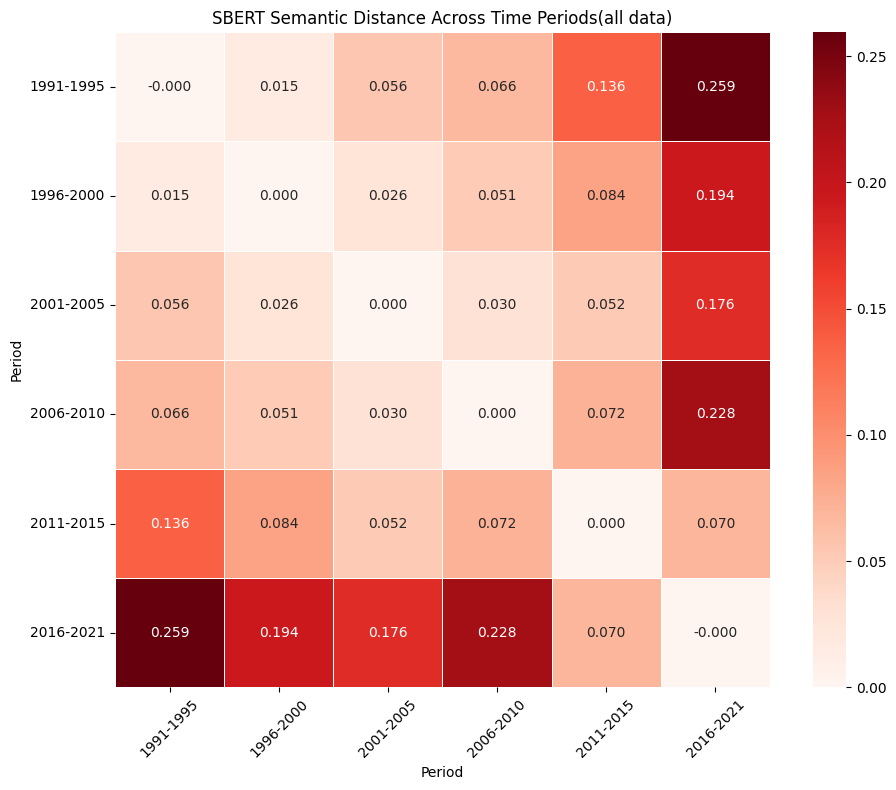
\includegraphics[width=0.9\linewidth]{figures/sbert_distance.png}
\caption{SBERT semantic distance across time periods.}
\label{fig:sbert_distance}
\end{figure}

In terms of LDA, mean topic proportions were used to compare thematic structure across periods. As described in the Methods section, $K=15$ was selected using coherence, and each period was represented by the average distribution of its vectors according to the topic. The results also support the hypothesis that LDA reveals structural reorganizations in research themes more clearly than TF-IDF. While TF-IDF identifies individual words that rise or decline, LDA groups related vocabulary into shared latent topics, making it easier to observe broader shifts in the focus of research. As shown in Figure~\ref{fig:lda_topic_trends}, Topic 8, associated with parsing, grammar, and syntactic structure, declines over time. In contrast, Topic 6, associated with neural architectures, attention, and transformers, increases strongly in later periods, showing that the research towards model is increasingly important. Topic 11, related to sentiment, social media, and bias detection, also becomes more visible after 2006-2010, while Topic 1, related to machine translation and multilingual NLP, remains comparatively stable, suggesting that some classic NLP tasks continued across periods.

Overall, SBERT and LDA support the TF-IDF finding that NLP shifted away from vocabulary relating grammar towards neural and model-related research. However, they add different evidence: SBERT shows smooth semantic drift, and LDA shows thematic reorganization behind the vocabulary shift. Additionally, their main limitation is explainability, because SBERT measures how much periods differ semantically, but not which terms caused the difference, while LDA topics need to be manually labeled from their top words.

\begin{figure}[t]
\centering
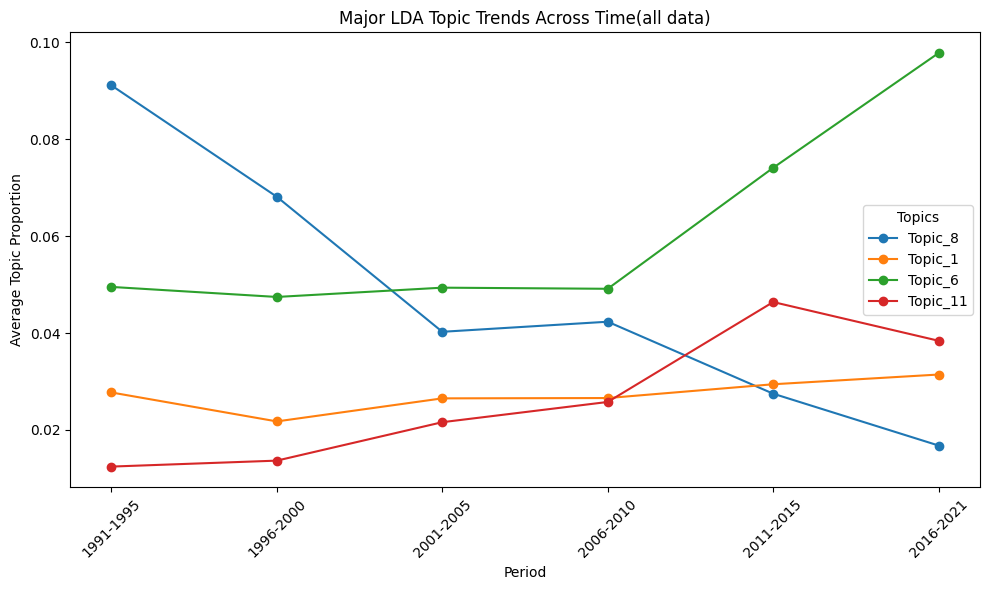
\includegraphics[width=0.9\linewidth]{figures/lda_topic_trends.png}
\caption{Major LDA topic trends across time periods.}
\label{fig:lda_topic_trends}
\end{figure}

% ── Member 5 supplement ──

\subsection{Axis 1: Trajectory Visualisation}
\label{sec:results-traj}

Figure~\ref{fig:pca-all} shows the centroid trajectories of the PCA for the four representations. The most significant characteristic is their convergence: regardless of whether the study is represented as vocabulary frequency, sentence embedding, or subject distribution, the maximum centroid shift occurs at the same transition point (Table~\ref{tab:traj-stats}). Stage from 2011-2015 to 2016-2021 dominated the total trajectory length in every panel, which is consistent with the emergence of pre-trained language models based on transformers after 2017\citep{pramanick_diachronic_2023}. This confirms the PCA hypothesis that a clear and consistent overall trajectory can be observed in all four representations.

\begin{figure*}[t]
 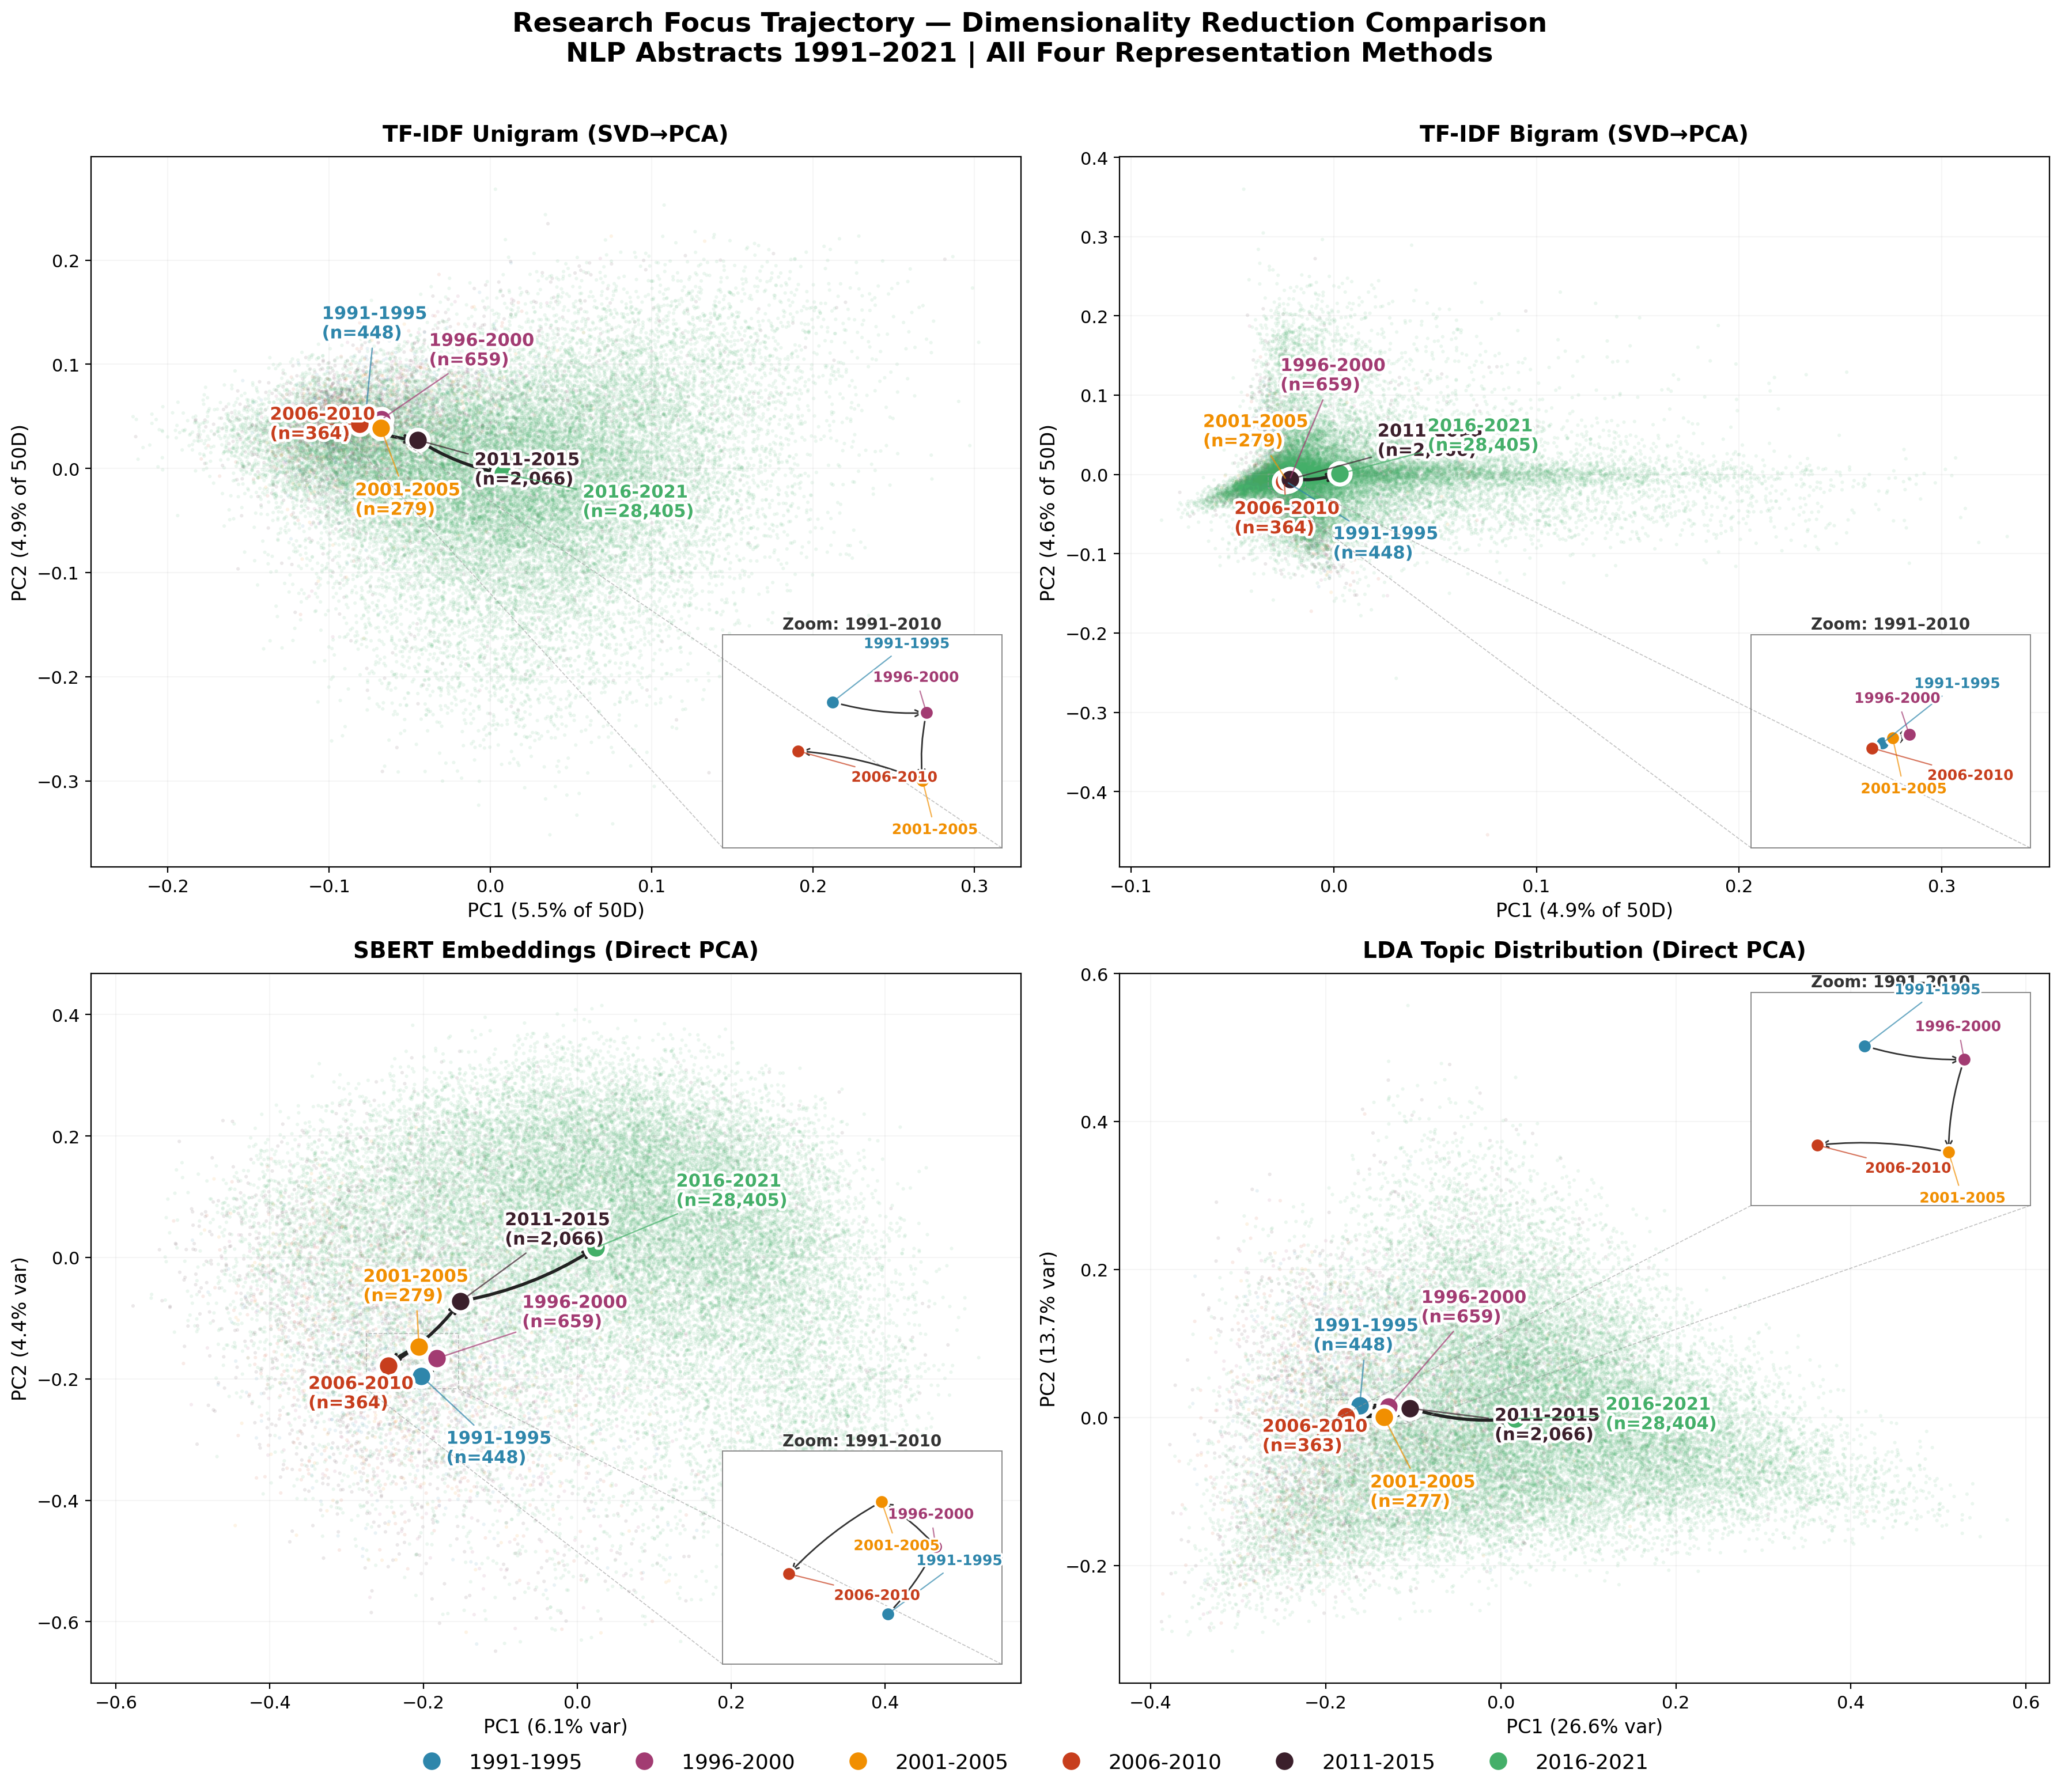
\includegraphics[width=\linewidth]{figures/pca_trajectory_all_methods_v3.png}
  \caption{PCA centroid trajectories (1991-2021) for all four
    Axis-1 representations. 
    Arrows connect consecutive 5-year period centroids.
    Zoomed insets reveal the 1991-2010 cluster, which is otherwise
    compressed by the scale of the 2016-2021 centroid
    ($n{=}28{,}405$; 88\% of the corpus).}
  \label{fig:pca-all}
\end{figure*}

\begin{table}[t]
  \centering\small
  \begin{tabular}{lccc}
    \hline
    \textbf{Method} & \textbf{Total} & \textbf{Max jump}
                    & \textbf{Period} \\
    \hline
    TF-IDF Unigram & 0.133 & 0.062 & 11-15$\,{\to}\,$16-21 \\
    TF-IDF Bigram  & 0.034 & 0.026 & 11-15$\,{\to}\,$16-21 \\
    SBERT          & 0.454 & 0.197 & 11-15$\,{\to}\,$16-21 \\
    LDA ($K{=}15$) & 0.286 & 0.122 & 11-15$\,{\to}\,$16-21 \\
    \hline
  \end{tabular}
  \caption{PCA centroid trajectory statistics (Euclidean distance in
    2D projected space).}
  \label{tab:traj-stats}
\end{table}

There are significant differences in displacement amplitudes between different methods. SBERT displayed the largest total trajectory (0.454) and single step (0.197), consistent with the results of Section~\ref{sec:results-sbert} that semantic embeddings capture a broader and more gradual drift than lexical methods.The total path of TF-IDF Bigram is much shorter (0.034 versus 0.133 for Unigrams), indicating that composite NLP terms are more stable than individual terms: sentences like \emph{language model} consolidate more quickly in the vocabulary than individual tokens containing relative frequency changes. The trajectory output of PCA is directly comparable across four panels because they share a common Euclidean scale. Compared to UMAP, this cross-method interpretability is a significant advantage, since the magnitude of the distance across the panels in UMAP is not linearly meaningful.

\begin{figure*}[t]
 \includegraphics[width=\linewidth]{figures/umap_trajectory_all_methods_v3.png}
  \caption{UMAP centroid trajectories for all four Axis-1 representations.}
  \label{fig:umap}
\end{figure*}

The UMAP projections corroborate the PCA consensus only partially: TF-IDF bigram and LDA agree with PCA on the 2011-2015 to 2016-2021 breakpoint, but TF-IDF unigram and SBERT under UMAP both peak one period earlier (2006--2010 to 2011-2015), indicating that distributional change registered earlier in lexical and semantic space than in the linear projection.

Across the four panels of Figure~\ref{fig:pca-all}, the three pre-transformer periods (1991-2010) cluster tightly while 2016-2021 sharply displaces to one side, which especially shows a clear plateau-then-jump structure in TF-IDF projections. Under SBERT and LDA, by contrast, the early periods trace a curved path: the early periods trace a curved arc that turns downward and rightward through 2011-2015 toward 2016-2021 under SBERT; under LDA the early-period path is similarly non-monotonic. This non-linearity, absent from TF-IDF, indicates that semantic and topical space was already reorganising during the machine-learning era (2001--2010) even as surface vocabulary remained stable, consistent with the staggered cosine
distance peaks in Section~\ref{sec:results-axis2}.

% ── Member 3: Axis 2A keyword shift results (Rubric 4a + 4b + 4c + 4d) ──
% Report and interpret the keyword shift results.
% Include figures and/or tables you think best present these findings.
% Analyse errors: where does keyword shift produce misleading results?
Mean TF-IDF scores were used as the primary metric, with $N = 20$ terms per period for both unigrams and bigrams. Mean normalisation was applied to account for corpus size imbalance. The early group consisted of 1991--1995, 1996--2000, and 2001--2005; the late group consisted of 2011--2015 and 2016--2021.

The results confirmed the hypothesis. Unigram analysis identified 14 emerging terms in the late periods, including \textit{neural}, \textit{learning}, \textit{models}, \textit{training}, and \textit{tasks}, none of which appeared in the top-20 lists of any early period. Against this, 20 terms disappeared, including \textit{grammar}, \textit{parsing}, \textit{unification}, \textit{syntactic}, and \textit{statistical}. Bigram analysis reinforced this pattern: \textit{deep learning}, \textit{pre trained}, \textit{language model}, and \textit{word embeddings} emerged in the late periods, while \textit{finite state}, \textit{tree adjoining}, and \textit{hidden markov} disappeared entirely. These findings are consistent with the TF-IDF results, which identify the same transition point, and align with documented developments in NLP history, including the Transformer architecture in 2017 and BERT in 2018 \citep{vaswani_attention_2023, devlin_bert_2019}.


\begin{figure*}[t]
\cnetering
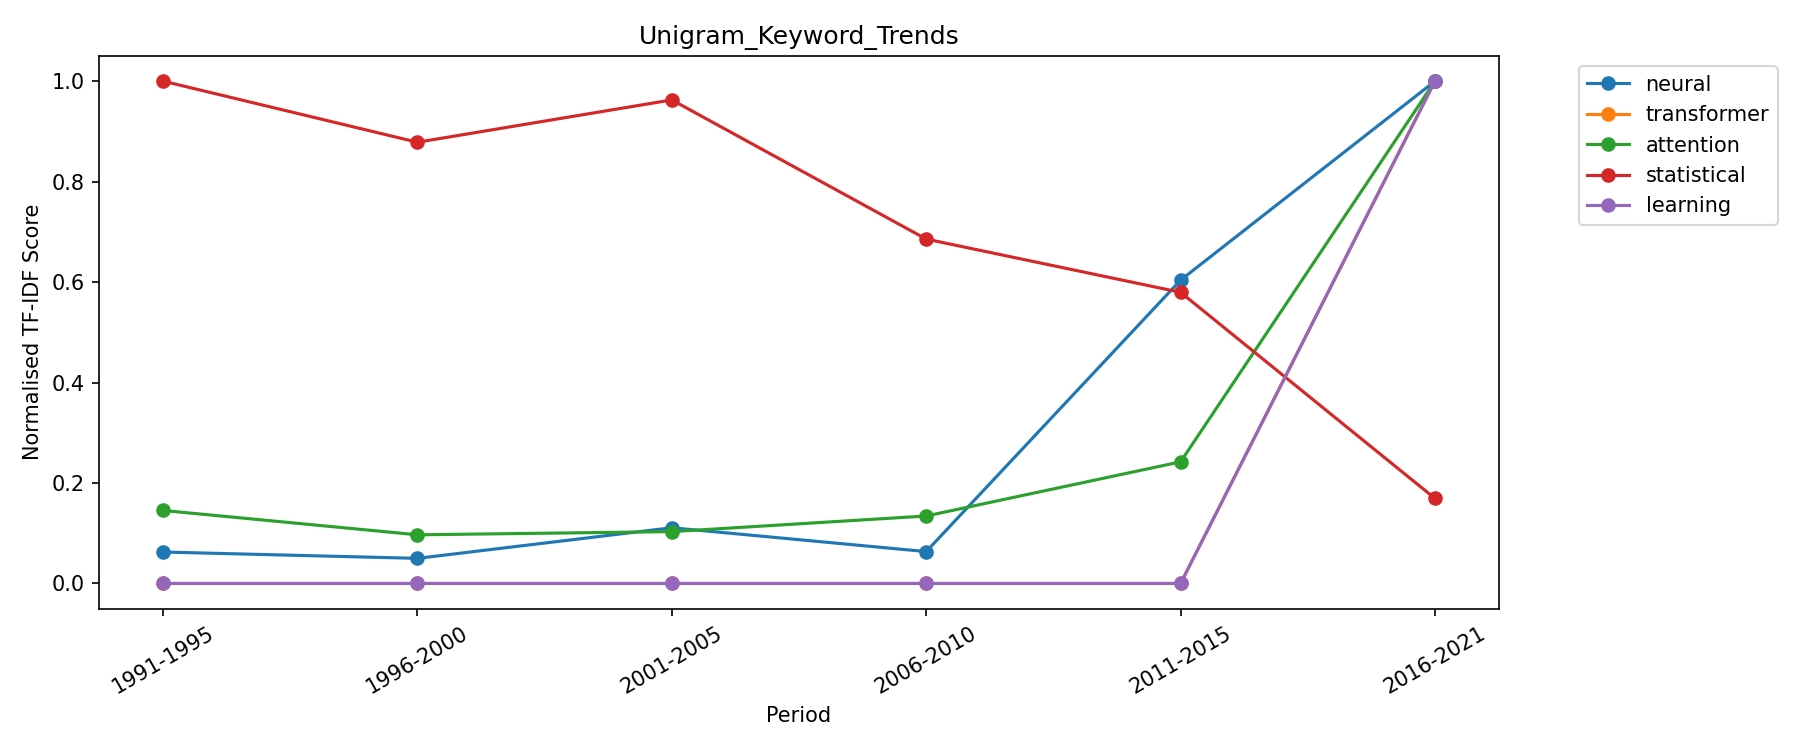
\includegraphics[width=\linewidth]
{figures/Unigram_Keyword_Trends.png}
\caption{Normalised TF-IDF scores for selected unigram terms across periods, showing the rise of neural vocabulary and decline of statistical and grammar-based terms.}
\label{fig:unigram_trends}
\end{figure*}


Keyword shift analysis offers high interpretability, as each finding traces directly to named vocabulary items. This contrasts with cosine distance, which quantifies the magnitude of change but cannot identify which terms drove it.

Two limitations apply. First, the method cannot distinguish genuine research shifts from changes in writing convention. Second, despite mean normalisation, the larger size of the 2016--2021 period may still cause its vocabulary to over-represent specialised subfields rather than field-wide trends. Despite these limitations, the results consistently indicate a major vocabulary shift beginning in the early 2010s, with 2006--2010 acting as a transitional phase.


% ── Member 4: Axis 2B cosine distance results (Rubric 4a + 4b + 4c + 4d) ─
% Report and interpret the cosine distance results.
% Include figures and/or tables you think best present these findings.
% Analyse errors: where does cosine distance produce misleading results?

\subsection{Axis 2B: Cosine Distance Analysis}
\label{sec:results-axis2}

The primary measure used in this analysis is cosine distance, it is defined as $1 - \cos(\theta)$ where $\theta$ is the angle between the two centroid vectors. A cosine distance value of 0 implies identical period representations, whereas a value of 1 indicates maximum divergence. This is best suited for high dimensional text vectors as it isn't  dependent on vector magnitude, meaning differences in abstract count across periods do not artificially inflate the measured change. However, centroid averaging compresses the full distribution of abstracts within a period into a single representative vector, potentially masking internal heterogeneity within a period.

Cosine Distance was computed on four representations: TF-IDF unigram, TF-IDF bigram, SBERT embeddings and LDA topic distributions, all developed from the full 32,217 abstract corpus. For each representation, one centroid vector was computed per period by taking the mean of all abstract vectors within that period. Distances were then calculated between every pair of adjacent periods, resulting in five transition scores across 1991 - 2021, All four representations were verified to share identical indices prior to analysis, confirming no alignment issues between the matrices.

\begin{table}[h!]
    \centering\small
    \begin{tabular}{lccc}
        \toprule
        \textbf{Transition} & \textbf{Unigram} & \textbf{Bigram} & \textbf{SBERT} & \textbf{LDA}  \\
        \midrule
        1991-1995 to 1996-2000 & 0.0763 & 0.3397 & 0.0152 & 0.087 \\
        1996-2000 to 2001-2005 & 0.1117 & 0.4381 & 0.0263 & 0.0092 \\
        2001-2005 to 2006-2010 & \textbf{0.1295} & \textbf{0.5482} & 0.0302 & 0.0106\\
        2006-2010 to 2011-2015 & 0.1127 & 0.4466 & \textbf{0.0721} & 0.0353\\
        2011-2015 to 2016-2021 & 0.0845 & 0.2449 & 0.0698 & \textbf{0.0639}\\
        \bottomrule
    \end{tabular}
    \caption{Cosine Distances between adjacent period centroids for TF-IDF unigram, TF-IDF bigram, SBERT and LDA representations}
    \label{tab:cosine-distances}
\end{table}

The above table, table~\ref{tab:cosine-distances} reports the cosine distances for all period transitions across all four representations. TF-IDF unigram distances range from ~0.075 to 0.13, bigram distances range from ~0.25 to 0.55 and SBERT distance range from ~0.015 to 0.072. TF-IDF unigram and bigram both identify the 2001-2005 to 2006-2010 transition as the largest shift, while SBERT identifies 2006-2010 to 2011-2015 as the biggest semantic change, one period later. LDA identifies 2011-2015 to 2016-2021 as the biggest topic-level shift, Highlighted in bold in the above table.

\begin{figure}[h!]
    \centering
    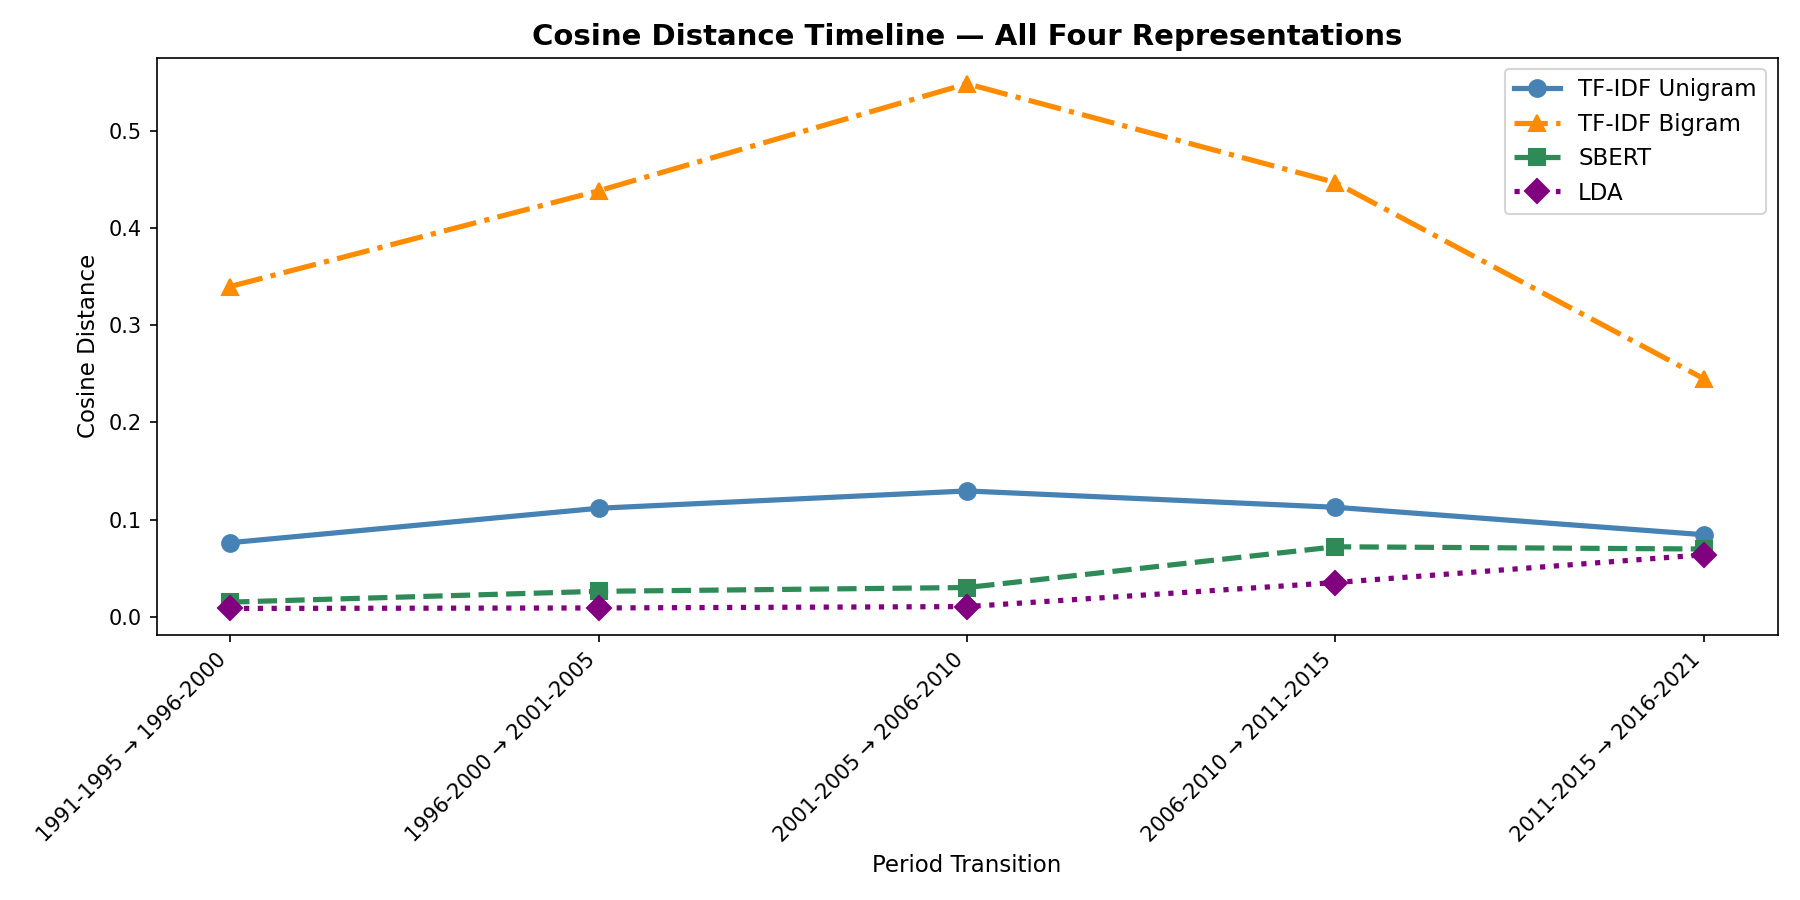
\includegraphics[width=\linewidth]{figures/cosine_distance_comparison.png}
    \caption{Cosine distance for TF-IDF unigram, TF-IDF bigram and SBERT representations across adjacent period transitions.}
    \label{fig:cosine-comparision}
\end{figure}

Figure~\ref{fig:cosine-comparision} shows all four timelines side by side. Notably, bigram distances are consistently larger than unigram distances across all transitions, confirming that domain-specific phrases are more era-specific than individual words.

Three limitations affect the reliability of these results. Firstly the corpus is heavily imbalanced: the 2016 - 2021 period has around 28,405 abstracts compared to 277 in 2001 - 2005. This means the 2016-2021 centroid is computed from vastly more data, potentially underestimating the true magnitude of change entering the transformer era. Second, SBERT distances are consistently smaller than TF-IDF distances across all transitions, which could reflect genuine semantic continuity or could indicate that the pre trained SBERT model encodes a modern NLP bias. Third LDA distances are the smallest overall, suggesting broad research topics shift more slowly than vocabulary or semantic meaning, however with only 15 topics the model may be too coarse to detect finer grained thematic transitions.

% ── Member 5: Discussion, strengths, limitations (Rubric 4e) ─────────────
% Synthesise all findings. Compare Axis 1 methods with each other.
% Compare Axis 2 methods with each other.
% State which method best balances consistency and interpretability.
% Discuss limitations of the overall approach.
% Add an evaluation table if you think it clarifies the comparison.

\subsection{Evaluation and Discussion}
\label{sec:eval-disc}

%\paragraph{Consistency across methods.}
The most robust finding of this study is the unanimous agreement on timing. All four Axis-1 representations identify the 2011-2015 to 2016-2021 transition as the dominant breakpoint under PCA (Table~\ref{tab:traj-stats}), and the keyword shift analysis in Section~\ref{sec:results-axis2} confirms the same period as the point at which neural and transformer vocabulary fully displaced statistical terminology.

Directional analysis identified a cluster of three. TF-IDF unigram (-31.9°), LDA at (-5.7°) and TF-IDF bigram (19.4°) are closely clustered together, while SBERT is located at 42.9° sitting apart from this cluster with WEAK agreement with unigram (74.8°). This pattern reflects a representational divide. TF-IDF and LDA both operate on vocabulary-level structure while SBERT's sentence-level embeddings capture a different dominant variance axis. Despite this directional divergence, the breakpoint consensus in Table~\ref{tab:traj-stats} stands as the primary, more robust finding.

Axis-2 cosine distance results showed extra temporal details. TF-IDF cosine distance reaches its peak at 2001-2005 to 2006-2010, SBERT peaks at 2006-2010 to 2011-2015, and LDA peaks at 2011-2015 to 2016-2021. It suggests that NLP's paragigm shift spreads upward through representational layers. Vocabulary first, semantic meaning second, thematic structure last. The NLP's semantic and topical space was already reorganising during 2001-2010, even as its lexical space remained stable.

%\paragraph{Interpretability.}
In terms of outputs communication, these methods are very different. Keyword shift analysis and TF-IDF produce specific lists of words that any reader can verify. Cosine distance quantifies magnitude but not source. LDA requires manual inspection of topic-word distributions. SBERT trajectories require probing experiments. Within the same method, we can at least compare PCA centroid positions across panels and use UMAP to qualify structural observation. For non-specialist communication, TF-IDF and keyword shift provide the best balance.SBERT is preferred to catch hidden semantic changes where vocabulary is stable. 

%\paragraph{Alignment with known NLP history.}
The 2011-2015 to 2016-2021 breakpoint matches the appearance of Transformer architecture (2017) and BERT and GPT-style pre-training (2018) \citep{pramanick_diachronic_2023, hall_studying_2008}. The earlier TF-IDF cosine peaks at 2011-2005 to 2006-2010 also map to the displacement of rule-based methods by SVMs and CRFs. \citep{hall_studying_2008}.

\begin{table}[t]
  \centering\small
  \begin{tabular}{lccc}
    \hline
    \textbf{Method} & \textbf{Cons.} & \textbf{Interp.}
                    & \textbf{Align} \\
    \hline
    TF-IDF Unigram  & H & H & H \\
    TF-IDF Bigram   & H & H & H \\
    SBERT           & H & L & H \\
    LDA             & H & M & H \\
    Keyword shift   & H & H & H \\
    Cosine distance & M & M & H \\
    PCA             & H & M & H \\
    UMAP            & M & L & M \\
    \hline
  \end{tabular}
  \caption{Method evaluation on three criteria (H\,=\,High,
    M\,=\,Medium, L\,=\,Low). Consistency (Cons.) reflects breakpoint agreement; interpretability (Interp.) reflects
    whether output identifies the source of change; alignment (Align.) reflects historical correspondence with documented NLP paradigm changes.}
  \label{tab:eval}
\end{table}



% ═══════════════════════════════════════════════════════════════════════════
% 4. CONCLUSIONS   Target: ~600 words total | ~120 words per member
%    Rubric: key findings, what worked, what did not, open challenges
% ═══════════════════════════════════════════════════════════════════════════
\section{Conclusions}
\label{sec:conclusions}

% Each member writes one paragraph (~120 words) addressing:
%   • The key finding from their axis/method
%   • One specific open challenge they identified
% Member 5 also writes a brief synthesis paragraph (~120w) to open and close.

% ── Member 5: opening synthesis (first paragraph) ─────────────────────────

The biggest shift supported by all four Axis-1 representation methods in NLP research occurred at the 2011-2015 to 2016-2021. Beneath this consensus, the Axis-2 cosine distance results show a layered pattern. TF-IDF peaks first, SBERT peaks one period later, and LDA is the last. Therefore, the shape of NLP's transformation depends on the metric. Cosine distance shows a rolling change. PCA shows a single break. We can only see the full picture by combining both axes. A gradual multi-layered reorganization that consolidated into a sharp, representation-agnostic shift at the dawn of the transformer era.

% ── Member 1: TF-IDF findings + open challenge ───────────────────────────
\TODO{Member 1 — (~120w).
What the TF-IDF analysis revealed about NLP's evolution.
Name one open challenge: e.g. how to handle vocabulary change
that is driven by synonyms rather than new terms.}{120}

TF-IDF analysis reveals how NLP research vocabulary has evolved, showing a decline in statistical terminology, a transitional phase around 2006-2010, and a rapid rise of neural and pre-training related terms after 2011.

The bigram representation refines this picture by capturing paradigm compound expressions that are not visible in unigram analysis. Both representations identify the same transition point, suggesting a robust structural change in the field.

A remaining limitation is the inability of TF-IDF to account for semantic continuity when terminology changes. Addressing this issue requires representations that operate beyond surface-level tokens, motivating the use of semantic models such as SBERT.


% ── Member 2: SBERT + LDA findings + open challenge ──────────────────────
SBERT and LDA extend the TF-IDF findings by showing that NLP's evolution was not only a vocabulary shift, but also a semantic and thematic reorganization. 

SBERT indicates gradual semantic drift across the full periods, while the relatively close distance between 2011-2015 and 2016-2021 suggests that the era of transformer research built on earlier deep learning patterns. LDA supports this by showing a decline of themes related to
parsing, grammar, and syntactic-structure themes, as well as the rise of themes related to neural architectures, attention, and transformers.

In general, these methods show that the change of vocabulary reflects broader changes in research meaning and thematic composition. One open challenge is explainability: the movement within the embedded space is difficult to explain without investigating, and LDA topic labels require manual judgement.


% ── Member 3: Keyword findings + open challenge ───────────────────────────

Keyword shift analysis revealed a sharp vocabulary transition at the 2011--2015 to 2016--2021 boundary. Terms associated with rule-based and statistical methods, including \textit{grammar}, \textit{parsing}, and \textit{unification}, declined steadily and were absent from late-period top-$N$ lists, while neural-era terms including \textit{neural}, \textit{training}, and \textit{language model} were absent before 2011 and dominant thereafter. The method's key strength is specificity: it names the words that changed, not only the fact that change occurred. A remaining open challenge is determining whether a rising term signals a genuine shift in research direction or a change in writing convention, as term frequency alone cannot separate scientific transition from linguistic trend.


% ── Member 4: Cosine distance findings + open challenge ───────────────────

Cosine distance analysis showed that the NLP shift over the years depends on which representation is used to measure it. Applied among four representations, TF-IDF unigram and bigram both indicated the largest vocabulary shift from period 2001-2005 to 2006-2010, SBERT identified the shift one period later 2006-2010 to 2011-2015, and LDA identified the shift one period later 2011-2015 to 2016-2021. This shows that NLP's transformation was not a sudden revolution but a gradual shift, surface vocabulary changed first, followed by semantic meaning, followed by a full reorganization of research topics. One open challenge remains: the corpus is heavily imbalanced, with 88\% of abstracts concentrated in the 2016--2021 period. This raises the question of whether the detected shifts reflect field-wide transitions or are partly an artefact of the growing volume of abstracts in recent years inflating the stability of later period centroids.

% ── Member 5: forward look (final paragraph) ──────────────────────────────

In practice, the best methods balanced sensitivity with clear communication. Looking at our whole pipeline, no single method gave us the complete picture. We got our strongest findings by triangulating across representations and comparing metrics. In lexical space, NLP's pre-transformer history looks like a stable plateau ending in a sudden break. But in semantic and topical space, it appears as a continuous non-linear reorganization. We can only see the cascade pattern in cosine distance by putting all four methods together.

% ═══════════════════════════════════════════════════════════════════════════
% REFERENCES  (not counted in the 10-page limit)
% Add BibTeX entries to references.bib and cite with \citep{} or \citet{}
% ═══════════════════════════════════════════════════════════════════════════
\bibliographystyle{acl_natbib}
\bibliography{custom}

\end{document}
